\section{Aufbau}
Grundsätzlich wird für den Versuch ein kompakter Wärmekonduktionsapparat mit vier Metallen verwendet.
Die Probenstäbe bestehen aus Aluminium, Edelstahl, sowie zwei unterschiedlich dicken Messingstäben. An jeweils beiden Enden des jeweiligen Stabes wird die Temperatur durch Thermoelemente abgegriffen. Der Abstand zwischen den einzelnen Thermoelementen beträgt $\increment x = \SI{0.03}{\meter}$. Für die Erwärmung der Stäbe wird ein Peltier-Element verwendet, welches mittig in der Apparatur verbaut ist. Die Temperaturen lassen sich über ein Temperatur Array mit einem Datenlogger verbinden welcher die Messwerte simultan aufnimmt. Die angeschlossene Spannung durch ein Spannungsgerät und die Abtastraten werden je nach Durchführungsmethode variiert. Der Aufbau ist in Abbildung \ref{fig:1} dargestellt und die Abmessungen der Stäbe, sowie die Literaturwerte für die Dichten $\rho$ und spezifischen Wärmen $c$ sind in Tabelle \ref{tab:lit} notiert.

\begin{figure}
    \centering
    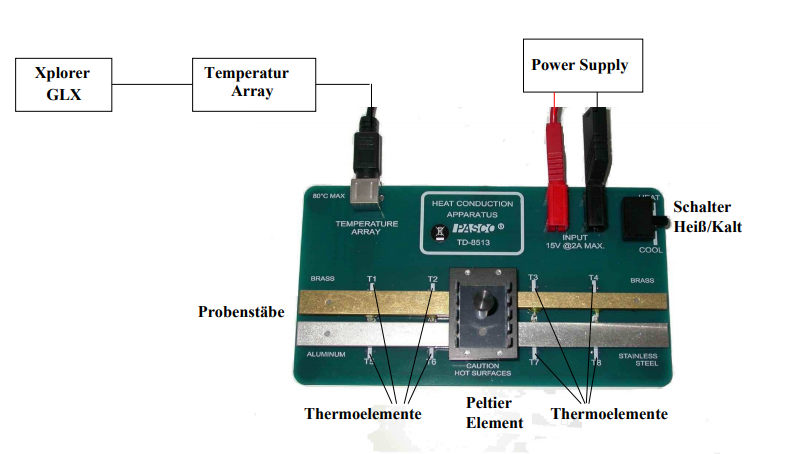
\includegraphics[width=\textwidth]{bilder/1.png}
    \caption{Aufbau des Wärmekonduktionsapparates. \cite{skript}} 
    \label{fig:1}
\end{figure}
\section{Versuchsdurchführung}
Es wurden zwei verschiedene Methoden verwendet um die Temperaturverläufe und dadurch die Wärmeleitfähigkeit $\kappa$ zu bestimmen. Diese sind im Folgenden erläutert.

\subsection{Statische Methode}
Zunächst sollte überprüft werden ob alle acht Temperaturen $T_{1}$ bis $T_{8}$ auch von dem Datenlogger angezeigt werden. Durchgeführt wird hier eine Messung mit einer angelegten Spannung von $U = \SI{5}{\volt}$ und einer Abtastrate von $\increment t = \SI{5}{\second}$. Das bedeutet es werden fünf Messungen pro Sekunde aufgezeichnet. Sobald die Spannung anliegt wird der Temperaturregler an der Apparatur \ref{fig:1} auf \enquote{HEAT} gestellt und die Stäbe werden während der Erhitzung von außen isoliert. Nach $\SI{700}{\second}$ wird die Messung beendet und die Werte lassen sich abspeichern.
Nach der Messung wird die Isolierung entfernt und der Schalter auf \enquote{COOL} zurückgestellt um die Stäbe für die nächste Messung wieder abzukühlen.
Mit diesen Temperaturwerten lassen sich nun Temperaturkurven erstellen und vergleichen, sowie Wärmeleitfähigkeiten $\kappa$ bestimmen.
\subsection{Dynamische Methode}
Bei der dynamischen Methode, auch Ångström-Methode genannt, werden die Metallstäbe periodisch immer wieder für eine feste Zeit erwärmt und dann abgekühlt. Die gewählte Periodendauer beträgt $T = \SI{200}{\second}$, dass heißt es wird $\SI{100}{\second}$ geheizt und dann $\SI{100}{\second}$ gekühlt.  Hierbei wird die Abtastrate auf $\increment t = \SI{2}{\second}$ reduziert und die Spannung auf $U = \SI{8}{\volt}$ erhöht.
Die Werte lassen sich wieder mit dem Datenlogger aufzeichnen und anschließend abspeichern.

